\section{Research Summary}

In this thesis, we explored various factors and aspects, all converging to answer the \textbf{Main Research Question}:

\mainrq

This question is encapsulated in Figure \ref{fig:wholepic}, where all the factors are presented as interconnected components within a larger system. This system embodies the fitness assessment process for sport horses during exercise through the analysis of data from non-invasive tools, encompassing both biomechanical and physiological aspects.

To elucidate Figure \ref{fig:wholepic}, we consider a scenario where we have data solely from an \gls{imu} mounted on the limb or the sacrum. This represents the non-invasive process of the assessment, where a lightweight \gls{imu} is affixed to the body using specialized tapes and fixtures, eliminating the need for invasive methods such as drawing blood using needles. The \gls{imu} data undergoes preprocessing to extract signal-based features, as demonstrated, for example, in Chapter \ref{chapter:Speed}. Gait events are essential for the computation and estimation of important fitness parameters, which are estimated with high accuracy. Subsequently, spatio-temporal parameters and biomechanical metrics per stride are derived. Leveraging this feature set, the rider classification model can accurately determine whether there is a rider on the horse. If no rider is detected, it prompts an assessment of the horse's fatigue status, indicating the need for rest. However, if the horse is being ridden, the system proceeds to estimate the \gls{lac} level, which translates into the horse's fatigue level. Based on this information, the rider, trainer, or veterinarian can reliably make informed decisions regarding whether to continue the exercise for fitness improvement or halt it to prevent potential injury. In summary, the multimodal system's process for estimating the fatigue level of sport horses was illustrated using an example.

\begin{figure}[!htb]
\centering
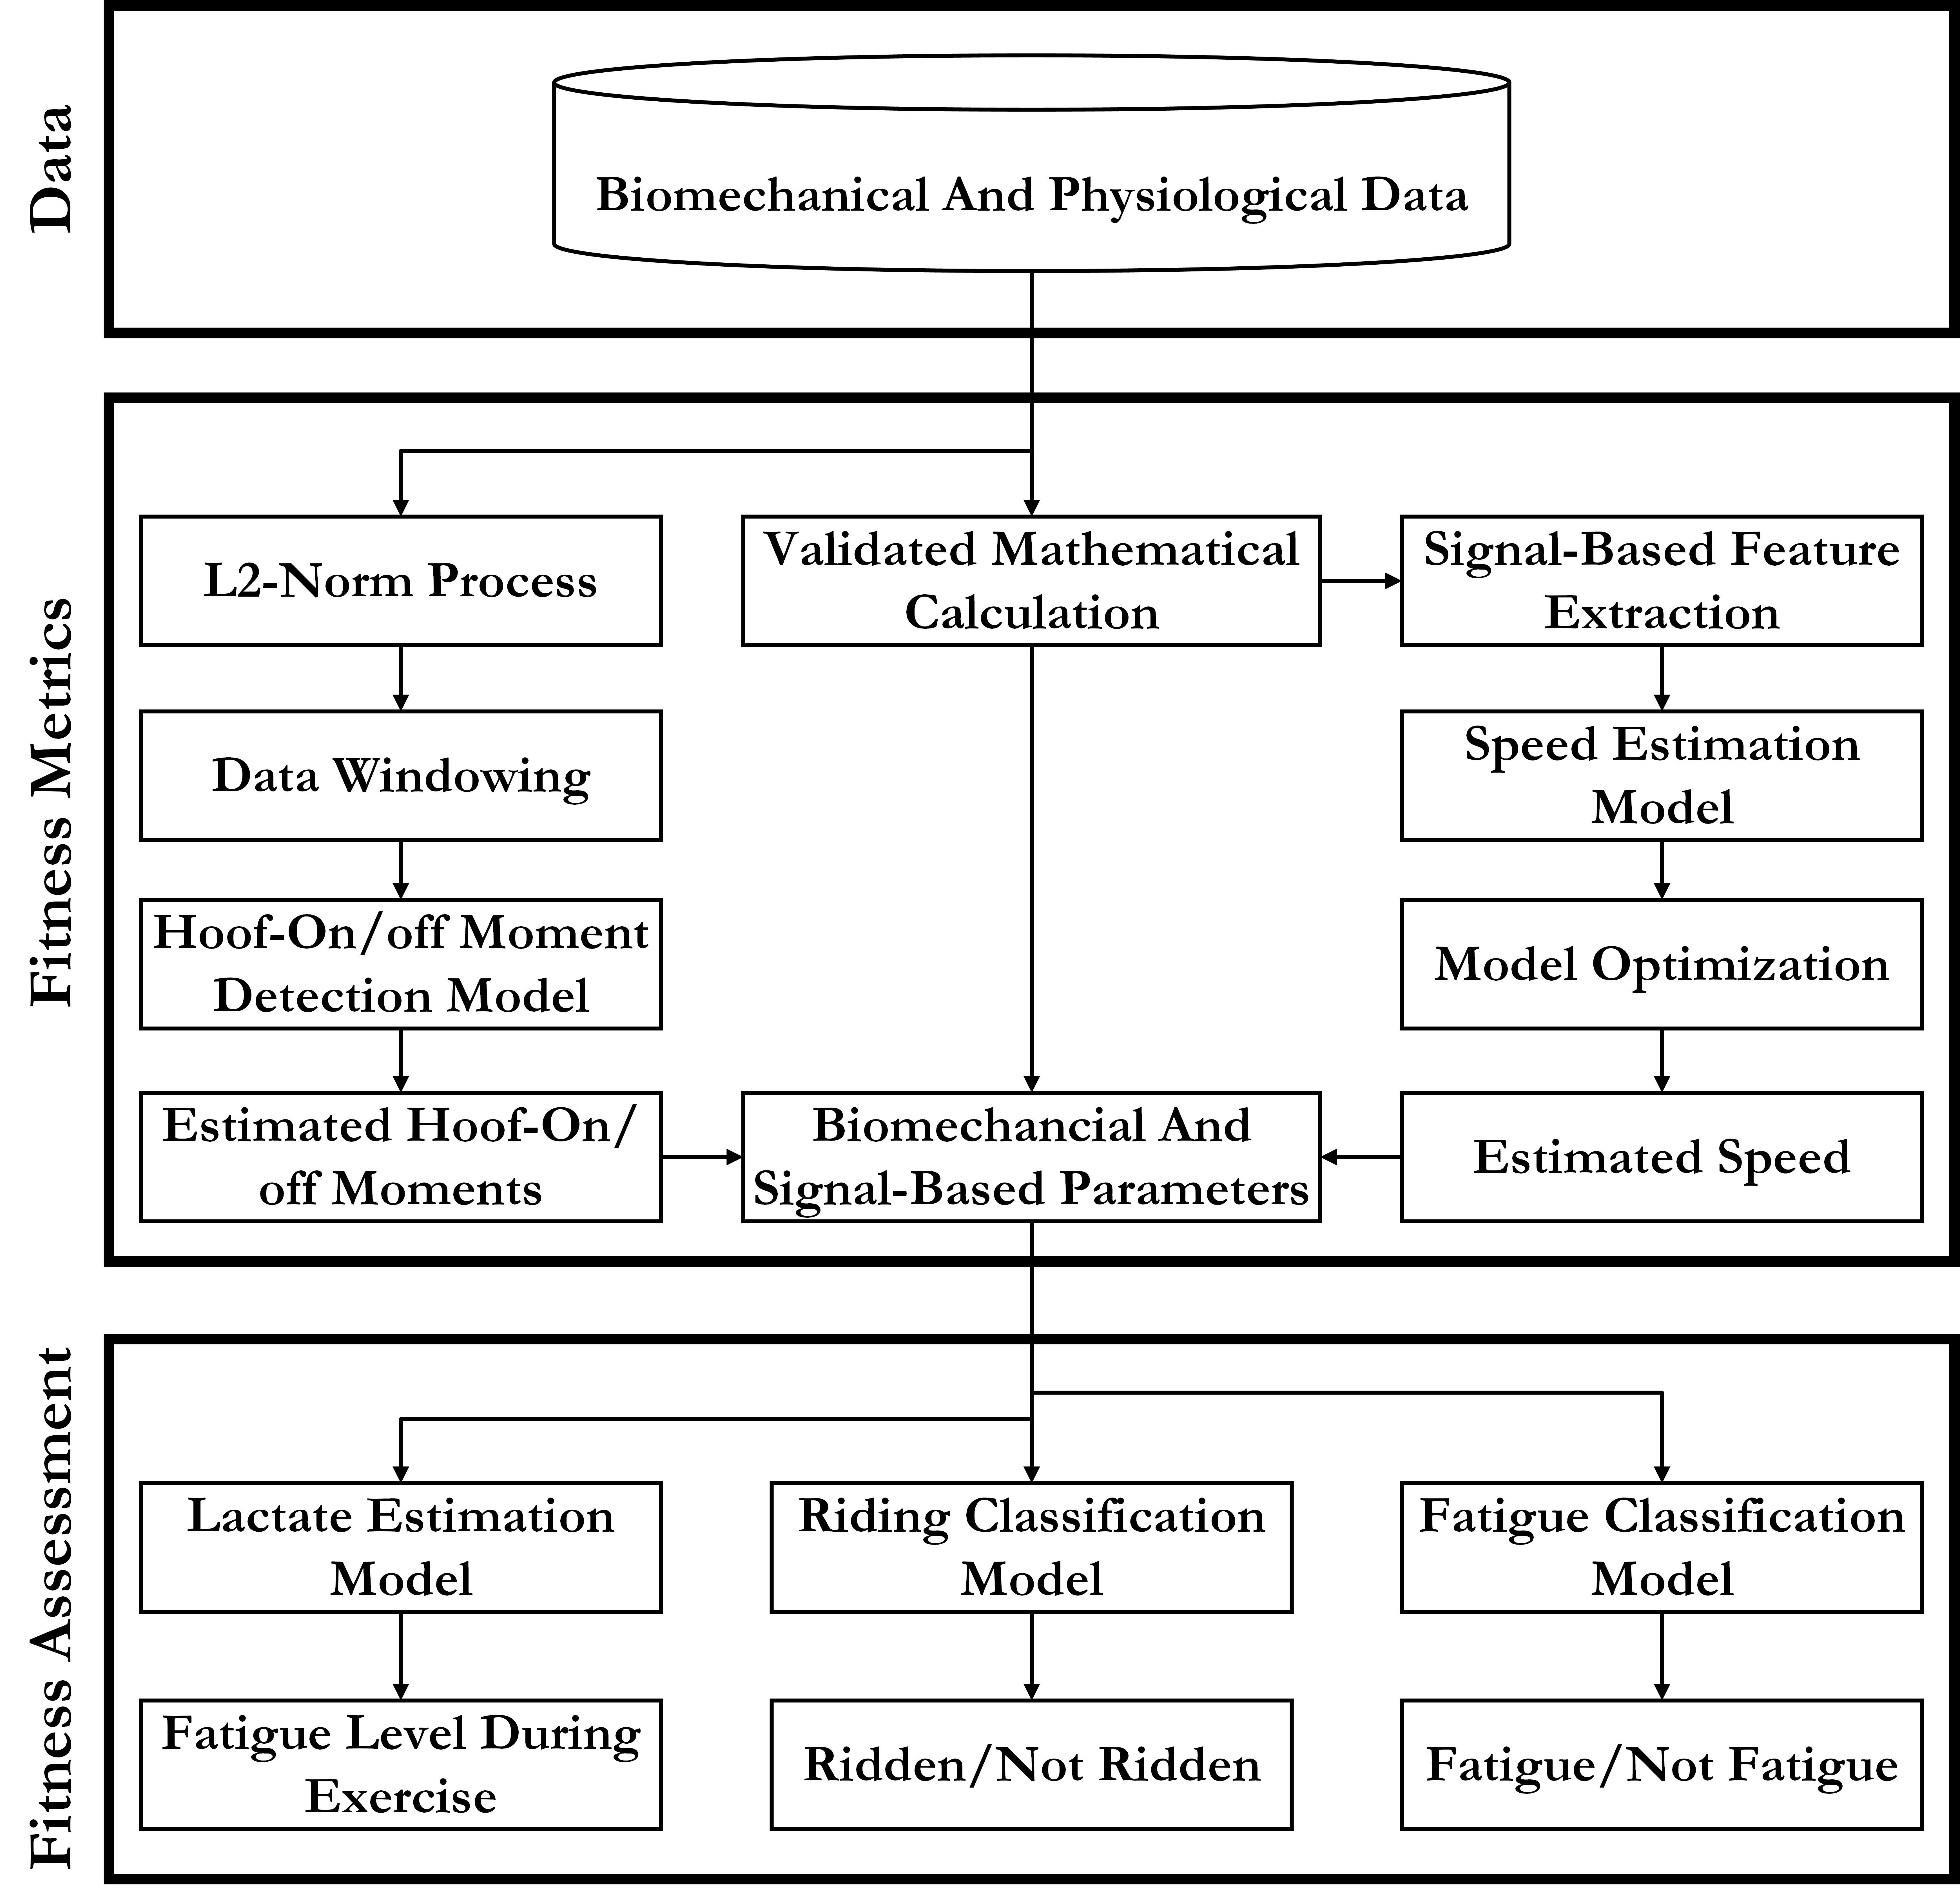
\includegraphics[width=\linewidth]{chapters/conclusions_future_work/figures/wholepic.png}
\caption{{\bf Thesis as an integrated multimodal system}}
\label{fig:wholepic}
\end{figure}

The five \textbf{Research Questions} that were introduced in Chapter \ref{sec:intro_research_objective} have been investigated throughout this thesis. This exploration has yielded several outcomes to the scientific literature, outlined as follows:

\vspace{0.3cm}

\noindent\textbf{\large The Prerequisite for Answering The Research Questions} 

\vspace{0.15cm}

\noindent\textbf{The outcome: Datasets}

One of the essential requirements that posed a challenge in addressing both the main research question and all the sub-questions was the need for a well-tailored dataset. In Chapter \ref{chapter:data}, we detailed the process of collecting data from various disciplines of sport horses during their training sessions. Since all the questions revolved around sport horses, it is important to note that every sport horse competes in a specific discipline. To ensure a comprehensive approach, we gathered data from sport horses across different disciplines.

We aimed to assess the fitness of the horses and sought to gather data that accurately represented their fitness levels. To achieve this goal, we employed \gls{set}, a set of tools accessible to trainers and veterinarians that can precisely measure a horse's fitness.

\vspace{0.3cm}

\noindent\textbf{\large Research Question 1:}

\textit{What are the key parameters that can determine the fitness of sport horses?}

\vspace{0.15cm}

\noindent\textbf{The outcome: Literature Review}

The equine literature was reviewed to identify important parameters relevant to fitness, whether for humans or sport horses. Specifically, we looked for parameters that significantly enhance or hinder the fitness of horses. The outcomes of the literature review are presented across three Chapters, particularly in the Introduction of Chapters \ref{sec:intro_introduction_step}, \ref{sec:intro_introduction_pelvis}, and \ref{sec:intro_introduction_speed}. According to the literature, the key parameters were related to spatio-temporal, gait events, and range of motion features.

\vspace{0.3cm}

\noindent\textbf{\large Research Question 2:}

\textit{What is the comparative reliability and accuracy between wearable sensors and traditional methods for measuring key fitness parameters?}

\vspace{0.15cm}

\noindent\textbf{The outcome: Validation of Measuring Device}

Since the foundation of the thesis relies on data obtained from a wearable device, we have chosen to maintain uniformity in the measuring device throughout all the studies. Therefore, we opted for an \gls{imu}, as detailed in Chapter \ref{chapter:data}. The \gls{imu} was selected owing to its suitability as a wearable device, high measurement accuracy, and capacity for real-time data acquisition. Although the \gls{imu} had been validated for measuring certain signals in the literature, it had not been validated for measuring the selected parameters required for fitness assessment. To address this, we conducted a validation study for the sensor's measurements of angles and displacements of various body parts, using \gls{omc} as the gold standard, as described in Chapter \ref{chapter:pelvis}. 

Furthermore, we validated the measurements of the \gls{gps} embedded in the \gls{imu} by comparing them to video camera recordings in Chapter \ref{chapter:Speed}. Additionally, we performed an extra validation of the speed estimation model based on the \gls{imu} data by testing it on an \gls{omc} dataset. All of the validation efforts concluded on the reliability of the \gls{imu}s used as the main device in this thesis.

\vspace{0.3cm}

\noindent\textbf{\large Research Question 3:}

    \textit{What approaches can be employed to measure key fitness parameters utilizing wearable sensors?}
\vspace{0.15cm}

\noindent\textbf{First outcome: Computational Resource Management}

Analyzing and processing complex machine learning models with numerous features typically demands substantial computational resources and a powerful computing machine, such as a standalone laptop. However, our goal was to identify models suitable for practical applications by riders and trainers. Therefore, in Chapter \ref{chapter:Speed} for speed estimation and Chapter \ref{chapter:rider} for riding state classification, we emphasized minimizing the required computational memory while ensuring that any reduction in accuracy did not significantly hinder the model's performance.

As an example, in Chapter \ref{chapter:rider}, by using only ten features out of the original 208, the model's accuracy decreased by 6.5\% but still remained at 90.9\%, which represents a high level of accuracy even with a substantial reduction in resource memory consumption. These results suggest the potential for real-time measurements by embedding the fitness assessment models into the sensors, allowing them to operate efficiently in low-memory environments.

\vspace{0.15cm}

\noindent\textbf{Second outcome: Versatility of Models}

Similar to human athletes, sport horses specialize in various disciplines, such as endurance, eventing, and dressage, each demanding a distinct set of skills. Additionally, certain horse breeds may exhibit superior performance in specific disciplines due to variations in their musculoskeletal structure. Furthermore, horses naturally and artificially execute different gaits, resulting in diverse movement patterns. Consequently, we trained our models to exhibit versatility in accommodating varying gait patterns, breeds, and disciplines. 

For instance, our versatile model for pre-\gls{set}/post-\gls{set} classification during both walk and trot performs at approximately the same level as a model focused solely on the trot (82\% versus 83\%), as shown in Table \ref{tab:variability_prepost}). Furthermore, when assessing the \gls{lac} estimation model with a discipline distinct from the one it was initially trained on (endurance versus eventers), we observed only a 4\% increase in error. This exemplifies the adaptability and versatility of our model, as illustrated in Figure \ref{results_fatigue_endur}.


\vspace{0.15cm}

\noindent\textbf{Third outcome: Modification and Optimization of Machine Learning Model}

While it was possible to apply the same machine learning algorithm across all models, we experimented with each problem. For every challenge addressed in this thesis, multiple machine learning and deep learning models were rigorously tested, and the one demonstrating the best performance was selected for the task. Moreover, particularly in cases where deep learning algorithms were employed (as seen in Chapters \ref{chapter:Step} and \ref{chapter:fatigue}), we conducted a systematic search to identify the optimal combination of hyperparameters for training the model.

Furthermore, when encountering class imbalances within the data, we took measures to address this issue. For example, in Chapter \ref{chapter:Step}, where there was a notable imbalance between hoof-on and hoof-off moments compared to other moments, we adapted the loss function to encourage the model to handle the output balance during its training.

\vspace{0.3cm}

\noindent\textbf{\large Research Question 4:}

\textit{How can machine learning models be developed for assessing the fitness of sport
horses?}

\vspace{0.15cm}

\noindent\textbf{The outcome: Integrating Biomechanical and Physiological Aspects}

Fitness encompasses a wide range of dimensions, such as psychological and nutritional aspects. In this thesis, our focus centered on aspects that can be quantitatively measured by sensors, narrowing our focus to two vital dimensions: biomechanical and physiological. Establishing a connection between these two dimensions was instrumental in enabling quantitative fitness assessment through sensor-derived data.

One of the primary motivations driving this thesis was the invasive and impractical nature of assessing fitness through physiological means only. Traditional methods often required drawing blood, necessitating exercise interruption, rendering them unsuitable for use in competitive environments where every second counts. Our success lies in translating the body's biomechanical responses into physiological metrics for fatigue assessment using machine learning algorithms.  The results demonstrated a minimal 8.72\% error when estimating \gls{lac} using biomechanical data. This estimation plays a pivotal role in identifying fatigue levels, thereby averting potential injuries and safeguarding fitness deterioration.

\vspace{0.3cm}

\noindent\textbf{\large Research Question 5:} 

\textit{How can the accuracy and reliability of the fitness assessment models be optimized for practical applications benefiting trainers, veterinarians, and riders?}

\vspace{.15cm}

\noindent\textbf{The outcome: Practicality of Using Wearable Sensors}

Many wearable sensors intended for human use in the commercial market are typically designed to be worn on the wrist. This design is primarily chosen for its convenience and accessibility. Nevertheless, it can potentially impact the precision of the gathered data. For example, studies have shown that employing a chest strap for heart rate monitoring and a sensor attached to the foot for tracking running balance and cadence yields more accurate results compared to the utilization of wrist-worn sensors. Therefore, we investigated the optimum number of \gls{imu}s and the best body location to place them for estimating the fitness parameters in terms of ease of use and accuracy in Chapter \ref{chapter:Step} for gait events, in Chapter \ref{chapter:Speed} for speed estimation, in Chapter \ref{chapter:rider} for riding status classification, and in Chapter \ref{chapter:fatigue} for \gls{lac} estimation.

In general, the inclusion of multiple wearable sensors on the body tends to enhance the accuracy of the models. Reducing the number of sensors to just one does not significantly impact overall accuracy; however, it necessitates a trade-off between practicality and precision.

When considering the use of only a single sensor for fitness evaluation, our research indicates that the sacrum proves to be a superior choice compared to alternative sensor placements, except for gait events estimation. Nevertheless, the practicality of attaching a sensor to the sacrum carries a risk of detachment. In terms of practicality, affixing sensors to the front limbs emerges as a more favorable option, as they can be securely wrapped around the distal limb for added stability.
